\documentclass[letterpaper]{article}
\usepackage{aaai}
\usepackage{times}
\usepackage{helvet}
\usepackage{courier}
\usepackage{xspace}
\usepackage{amssymb}
\usepackage{amsmath, esvect}
\usepackage{xspace, mathtools, comment}
\usepackage[para,online,flushleft]{threeparttable}
\usepackage{booktabs, multirow, soul}
\usepackage{natbib}
\usepackage{graphicx}
\usepackage{caption}
\usepackage{subcaption}
\frenchspacing
\setlength{\pdfpagewidth}{8.5in}
\setlength{\pdfpageheight}{11in}
\pdfinfo{
/Title (Insert Your Title Here)
/Author (Put All Your Authors Here, Separated by Commas)}
\setcounter{secnumdepth}{2}

\newcommand{\etal}{\mbox{\emph{et al.}}\xspace}
\newcommand{\R}{\mathbb{R}}

\newcommand{\mhcflurrynd}{\mbox{$\mathop{\mathtt{MHCflurry 2.0}}\limits$}\xspace}
\newcommand{\dynappo}{\mbox{$\mathop{\mathtt{DyNA\ PPO}}\limits$}\xspace}
\newcommand{\pepppo}{\mbox{$\mathop{\mathtt{PepPPO}}\limits$}\xspace}

\newcommand{\bpvae}{\mbox{$\mathop{\mathtt{BPVAE}}\limits$}\xspace}
\newcommand{\bovae}{\mbox{$\mathop{\mathtt{BOVAE}}\limits$}\xspace}
\newcommand{\mcts}{\mbox{$\mathop{\mathtt{MCTS}}\limits$}\xspace}
\newcommand{\random}{\mbox{$\mathop{\mathtt{Random}}\limits$}\xspace}
\newcommand{\pwm}{\mbox{$\mathop{\mathtt{PWM}}\limits$}\xspace}

\newcommand{\vect}[1]{\mathbf{#1}}
\newcommand{\matr}[1]{\uppercase{#1}}

\newcommand{\mhcfunc}{\mbox{$\mathop{f}$}\xspace}
\newcommand{\allele}{\mbox{$\mathop{m}$}\xspace}
\newcommand{\alleleemb}{\mbox{$\vect{m}$}\xspace}
\newcommand{\peptide}{\mbox{$\mathop{p}$}\xspace}
\newcommand{\blosum}{\mbox{$\mathop{\mathtt{BLOSUM}}\limits$}\xspace}
\newcommand{\len}{\mbox{$\mathop{l}$}\xspace}
\newcommand{\state}{\mbox{$\mathop{s}\limits$}\xspace}
\newcommand{\aminoset}{\mbox{$\mathcal{A}$}\xspace}
\newcommand{\amino}{\mbox{$\mathop{a}$}\xspace}
\newcommand{\aminoemb}{\mbox{$\vect{e}$}\xspace}
\newcommand{\hidden}{\mbox{$\vect{h}$}\xspace}
\newcommand{\cell}{\mbox{$\vect{c}$}\xspace}
  
 \begin{document}
% The file aaai.sty is the style file for AAAI Press 
% proceedings, working notes, and technical reports.
%                                                                                                                                                                                                                                                                                                                
\title{Mutating Peptides binding to MHC class-I molecules with Reinforcement learning}
\author{AAAI Press\\
Association for the Advancement of Artificial Intelligence\\
2275 East Bayshore Road, Suite 160\\
Palo Alto, California 94303\\
}
\maketitle
\begin{abstract}
\begin{quote}
Foreign peptides bound to major histocompatibility complex (MHC) class-I molecules and presented on the cell 
surface play a vital role in the immunotherapy.
%
These foreign peptides can be recognized by T-cell receptors to trigger the adaptive immune response.
%
In this paper, we formulate the identification of these foreign peptides as a reinforcement learning (RL) problem, 
and present a framework, which we call \pepppo, to generate peptides that can be presented by any given MHC molecules.
%
\pepppo learns to mutate any random peptides into positive peptides that can be presented 
on the cell surface by the given MHC molecule.
%
%\st{In addition to generating positive peptides, we design another constraint to require that the 
%generated peptides are dissimilar with the human peptides, and thus could potentially be  
%the candidates of peptide-based vaccines.}
%
The experiments show that our method can successfully generate positive peptides with high 
presentation scores predicted by the well-developed computational tools.
%
The generated peptides also have been validated by the physical models to be able to bind with the MHC molecules.
\end{quote}
\end{abstract}

%%%%%%%%%%%%%%%%%%%%%%%%%%%%%%%%%%%%%%%%%%%%%%%%%%%%%%%%%%%%%%%%%%%%%%%%%%%%%%%%%%%%%%%%%%%%%%%%%%%%%%%%%%%%
\section{Introduction}
\label{sec:intro}
%%%%%%%%%%%%%%%%%%%%%%%%%%%%%%%%%%%%%%%%%%%%%%%%%%%%%%%%%%%%%%%%%%%%%%%%%%%%%%%%%%%%%%%%%%%%%%%%%%%%%%%%%%%%

We summarize our contributions below:

1) We formulated the identification of positive peptides as a novel reinforcement learning problem. We built 
an RL environment from the well-developed computational tools and learned a policy to generate positive peptides
within the built environment.

2) Our method can generate positive peptides with large predicted presentation scores. The generated 
positive peptides are also validated to be able to bind with the MHC molecules by the physical models.

%\st{3) We designed a new constraint to generate peptides that are dissimilar with the human peptides and thus more 
%likely to be the candidates of peptide-based vaccines.}
3) We built a database of potentially positive peptides for all the known alleles using our method to accelerate 
the development of peptide vaccines.

4) We developed multiple different baseline methods and demonstrated the effectiveness of \pepppo with a detailed comparison.

%%%%%%%%%%%%%%%%%%%%%%%%%%%%%%%%%%%%%%%%%%%%%%%%%%%%%%%%%%%%%%%%%%%%%%%%%%%%%%%%%%%%%%%%%%%%%%%%%%%%%%%%%%%%
\section{Related Works}
\label{sec:related}
%%%%%%%%%%%%%%%%%%%%%%%%%%%%%%%%%%%%%%%%%%%%%%%%%%%%%%%%%%%%%%%%%%%%%%%%%%%%%%%%%%%%%%%%%%%%%%%%%%%%%%%%%%%%

To the best of our knowledge, Angermueller \etal \cite{angerm2020} first proposed a model-based reinforcement 
learning method based on proximal-policy optimization (PPO) named \dynappo, for the biological sequence design.
%
\dynappo 
and \cite{marcin2020}

%%%%%%%%%%%%%%%%%%%%%%%%%%%%%%%%%%%%%%%%%%%%%%%%%%%%%%%%%%%%%%%%%%%%%%%%%%%%%%%%%%%%%%%%%%%%%%%%%%%%%%%%%%%%
\section{Methods}
\label{sec:method}
%%%%%%%%%%%%%%%%%%%%%%%%%%%%%%%%%%%%%%%%%%%%%%%%%%%%%%%%%%%%%%%%%%%%%%%%%%%%%%%%%%%%%%%%%%%%%%%%%%%%%%%%%%%%

%===========================================================================================================
\subsection{Problem Definition}
\label{sec:method:problem}
%===========================================================================================================
%
In this paper, we focus on the generation of peptides presented on the cell surface by the MHC class I molecules.
%
We use a computational tool named \mhcflurrynd \cite{odonnell2020}, to estimate the presentation scores of peptides with an given
MHC molecule.
%
The presentation score is a composite score of the antigen processing (AP) prediction 
and the binding affinity (BA) prediction.
%
The AP prediction predicts the probability for a peptide to be delivered by the transporter associated with antigen processing (TAP) protein complex 
into the endoplasmic reticulum (ER), where the peptide can bind to MHC molecules.
%
The BA prediction predicts the binding strength between the peptide and MHC molecules.
%
Higher presentation scores require higher AP and BA scores, and indicate higher probabilities for generated peptides to be presented on the 
cell surface by the given MHC molecules.

\textbf{Problem Definition:} 
%
We represent a peptide as a sequence of amino acids $\{\amino_i\}^l$, where \amino is one of 20 types of natural amino acids and 
$l$ is the length of the sequence.
%
Given an MHC molecule \allele, \pepppo aims to generate a peptide $\peptide$ with $l$ amino acids that can maximize the presentation scores $r(\peptide, \allele)$
predicted by the \mhcflurrynd.
% 
%
%\st{In addition to the presentation score objective, another objective on human peptides $\{\peptide_H\}$ is also incorporated to 
%generate peptides that are dissimilar with the human proteins $\min(\{\text{dist}(\peptide, \peptide'),\ \forall \peptide' \in \{\peptide_H\}\}) < d_t$.
%%
%The distance function $\text{dist}(.,.)$ could be hamming distance or substitution distance with Blosum62 matrix, and $d_t$ represents the distance 
% threshold used to filter out generated peptides similar with human proteins.}
%

%===========================================================================================================
\subsection{Peptide Mutation Environment}
\label{sec:method:environment}
%===========================================================================================================

The peptide mutation environment consists of 3 components including the state space, the action space and the reward design.
% 
In this section, we discuss these 3 components of the peptide mutation environment as below.

\textbf{State Space:} 
We define the state of the environment $\state_t$ at time step $t$ as a pair of an MHC class I molecule and a peptide $(\peptide, \allele)$.
%
We represent an MHC molecule as a pseudo sequence with 34 amino acids, each of which is in potential contact with the bound peptide within a distance of 4.0 \AA, 
following the previous works for peptide-MHC binding prediction~\cite{Nielsen2007,Jurtz2017}.
%
With a peptide of length $\len$ and an MHC molecule, we represent the state $\state_t$ as a tuple $\state^t=(E^{\peptide}, E^{\allele})$, in which $E^{\peptide}$ 
and $E^{\allele}$ are the encoding matrices of the peptide and the MHC molecule, respectively.
%
The details of the encoding method will be described in Section~\ref{sec:method:encode}.
%
During the training, to initialize the state $\state^0$, we randomly sample an MHC class I molecule, and get a random initial peptide sequence with 50\% chance of 
randomly sampling from peptides in the IEDB dataset or with 50\% of randomly generating a new one.
%
We define the terminal state $\state_T$ as the state with the maximum time step $T$ or with the presentation score greater than threshold $\sigma$.

\textbf{Action Space:} 
We define a multi-discrete action space to optimize the peptide by replacing one amino acid with another one.
%
At time step $t$, given a peptide $\peptide^t=\{\amino_i\}^l$, the action is to first determine the position of 
the amino acid to be replaced, and then predict the type of new amino acid at the position. 

\textbf{Reward Design:} 
We only use the final rewards to guide the optimization of RL agents, that is, only terminal states can receive rewards from the peptide mutation environment.
%
We define the final rewards as the predicted presentation scores $r(\peptide, \allele)$ of \mhcflurrynd between the peptides $\peptide_T$ and the MHC molecules 
$\allele$ within the terminal state $\state_T$.

%===========================================================================================================
\subsection{Pan-allele Mutation Policy Network}
\label{sec:method:policy}
%===========================================================================================================
%represented with a mixture of multiple encoding methods 
%with the BLOSUM matrix, the one-hot vectors and the embedding matrix learned during the training.
%%
%This mixture of encoding methods has been demonstrated in \cite{Chen2021} to achieve the best prediction performance on peptide-MHC binding prediction among all
%the combinations of these encoding methods. 


In this section, we introduce our policy network learned by the RL agent to mutate the amino acids within the peptides given an 
MHC molecule.
%
Specifically, the policy network takes the peptide and the given MHC molecule as input and learns to mutate one amino acid 
in the peptide sequences at each step to maximize the presentation scores.
%
%At each step, the policy mutates the peptide by replacing one amino acid with another amino acid.

\textbf{Encoding of Amino Acids} We use a mixture of multiple encoding methods to represent the amino acids within the peptide sequences and the MHC molecules.
%
We represent each amino acid by concatenating the encoding vectors $\aminoemb^B$, $\aminoemb^O$ and $\aminoemb^D$ from the BLOSUM matrix, the one-hot matrix and 
the learnable embedding matrix, respectively, that is, $\aminoemb = \aminoemb^B \oplus \aminoemb^O \oplus \aminoemb^D$ and $\aminoemb\in\R^{d}$.
%
This method has been demonstrated in \cite{Chen2021} to achieve the best prediction performance on peptide-MHC binding prediction among all
the combinations of these encoding methods. 
%
The encoding matrices $E^{\peptide}$ and $E^{\allele}$ of the peptide \peptide and the MHC molecule \allele are then represented as 
$E^{\peptide}=\{\aminoemb_1,...,\aminoemb_l\}\in\R^{l\times d}$ and 
$E^{\allele}=\{\aminoemb_1,...,\aminoemb_{34}\}\in\R^{34\times d}$, respectively.

\textbf{Embedding of States} In order to predict the mutation of amino acids in peptide sequences, we first embed each amino acid $\amino_i$ within 
the peptide sequences $\{\amino_i\}^l$ into an continuous latent vector $\hidden_i$ using one-layer bidirectional LSTM as below,
%
\begin{equation}
\begin{array}{c}
\overrightarrow{\hidden}_i, \overrightarrow{\cell}_i = \text{LSTM}(\aminoemb_i, \overrightarrow{\hidden}_{i-1}, \overrightarrow{\cell}_{i-1}; \overrightarrow{\theta}^{\peptide})\\
\overleftarrow{\hidden}_i, \overleftarrow{\cell}_i = \text{LSTM}(\aminoemb_i, \overleftarrow{\hidden}_{i+1}, \overleftarrow{\cell}_{i+1}; \overleftarrow{\theta}^{\peptide})\\
\hidden_i = \overrightarrow{\hidden}_i \oplus \overleftarrow{\hidden}_i\\
\end{array}
\end{equation}
%
where $\overrightarrow{\hidden}_i/\overleftarrow{\hidden}_i$ is the hidden state vector of $i$-th amino acid; 
$\overrightarrow{\cell}/\overleftarrow{\cell}$ are the memory cell states of $i$-th amino acid;
$\overrightarrow{\hidden}_0$,$\overleftarrow{\hidden}_l$, $\overrightarrow{\cell}_0$ and $\overleftarrow{\cell}_l$ are initialized with random noise vectors;
$\overrightarrow{\theta}^{\peptide}$ and $\overleftarrow{\theta}^{\peptide}$ are the learnable parameters of LSTM of forward and backward direction, respectively.
%
With the embeddings of all the amino acids, we define the embedding for the peptide sequence as the concatenation of hidden vectors at two ends, 
that is, $\hidden^p = \overrightarrow{\hidden_l} \oplus \overleftarrow{\hidden_0}$.

To embed an MHC molecule into a continuous latent vector, we first flatten the encoding matrix $E^{\allele}$ into a vector $\alleleemb$.
%
Then, we learn the continuous latent embedding $\hidden^{\allele}$ with,
%
\begin{equation}
\hidden^{\allele} = W_1^{\allele}\text{ReLU}(W_2^{\allele}\alleleemb)
\end{equation}
%
where $W_i^{\allele}$(i=1,2) are the learnable parameter matrices.
%

\textbf{Action Prediction}
%
At time step $t$, we optimize the peptide sequence $\peptide_{t}$ by predicting the mutation of one amino acid
with the latent embeddings $\hidden^{\peptide_t}$ and $\hidden^{\allele}$.
%
Specifically, we first select the amino acid $\amino_i$ in $\peptide_{t}$ as the one to be replaced.
%
We then predict which amino acid should be used to replace $\amino_i$.
%
Inspired by~\cite{pardo2018}, we add the current time step $t$ as an additional feature into the prediction,
so that the agent can optimize the peptides within the time limit $T$.
%
We predict whether the amino acid $\amino_i$ should be replaced, with the score of replacement calculated as below, 
\begin{equation}
f^c(\amino_i) = (\vect{w}^c)^T(\text{ReLU}(W_1^c\hidden_i + W_2^c\hidden^{\allele} + w_3^ct))
\end{equation}
%
where $\hidden_i$ is the hidden latent vector of amino acid $\amino_i$ from LSTM;
%
$w_3^c$, $\vect{w}^c$ and $W_i^c$ (i=1,2) are the learnable scalar, vector and matrices, respectively.
%
The amino acid with the highest score will be selected to be replaced with another amino acid.
%
After determining the amino acid $\amino_i$, we predict the type of the amino acid used to replace $\amino_i$ as below,
\begin{equation}
f^d(\amino_i) = \text{softmax}(W_1^d \times \text{ReLU}(W_2^d\hidden_i+W_3^d\hidden^{\allele}+w_3^dt))
\end{equation}  
where $w_3^d$ and $W_i^d$ (i=1,2,3) are the learnable scalar and matrices, respectively;
$\text{softmax}(.)$ converts a vector into probabilities over 20 amino acid types.
%
Note that we will mask the original type of $\amino_i$ and replace $\amino_i$ with a different type of amino acid.

%===========================================================================================================
\subsection{Optimization}
\label{sec:method:optimization}
%===========================================================================================================

We leverage PPO \cite{schulman17ppo} to optimize the agent so that the peptides generated by the agent could have the 
maximum presentation score with a given MHC molecule.
%
The objective function of PPO is defined as below,
\begin{equation}
\max J(\theta) = 
\end{equation}


%%%%%%%%%%%%%%%%%%%%%%%%%%%%%%%%%%%%%%%%%%%%%%%%%%%%%%%%%%%%%%%%%%%%%%%%%%%%%%%%%%%%%%%%%%%%%%%%%%%%%%%%%%%%
\section{Experimental Settings}
\label{sec:experiments}
%%%%%%%%%%%%%%%%%%%%%%%%%%%%%%%%%%%%%%%%%%%%%%%%%%%%%%%%%%%%%%%%%%%%%%%%%%%%%%%%%%%%%%%%%%%%%%%%%%%%%%%%%%%%

%===========================================================================================================
\subsection{Baseline Methods}
\label{sec:experiments:baseline}
%===========================================================================================================
%
To demonstrate the effectiveness of the proposed \pepppo, we develop multiple baselines as below and compare our method with them.

\begin{itemize}
	\item \mcts: Monte Carlo Tree Search.
	      
	      Given an MHC molecule, \mcts generates peptide sequences by adding one amino acid step by step
	      until reaching the maximum length of 15 amino acids or with the presentation scores greater than a threshold.
	      %
	      All the generated peptides with no less than 8 amino acids will be evaluated by \mhcflurrynd.
	      %
	\item \bovae: Bayesian Optimization with the Variational Autoencoder.
	
	      In \bovae, a VAE model is pre-trained to convert peptide sequences of variable lengths into continuous latent 
	      embeddings of a fixed size.
	      %
	      Given an allele, the bayesian optimization algorithm with RBF kernel is then employed to optimize random latent embeddings 
	      with maximum $t$ steps so that the peptide sequences decoded from the optimized latent embeddings are with the high presentation scores.
	      %
	      At each step, \bovae evaluates the presentation scores of the generated peptides with \mhcflurrynd, and stop the optimization and 
	      output the peptides if their presentation scores are greater than a threshold.
	      %
	\item \bpvae: Back Propagation with the Variational Autoencoder.
		  
		  In \bpvae, a student model with the variational autoencoder same as that in the \bovae is employed to learn the presentation scores 
		  from \mhcflurrynd.
		  %
		  After getting the trained student model, \bpvae can generate peptides by optimizing the latent embeddings of peptides through 
		  gradient ascent to maximize the predicted presentation scores in the student model.
		  %
	      The decoded peptide sequences with $t$ steps will be evaluated by \mhcflurrynd.
	      %
	\item \pwm: Position weight matrix.
	
	      To derive the position weight matrix for each allele, we used the data set for \mhcflurrynd curated by \cite{odonnell2020} to 
	      infer the position weight matrices.
	      %
	      For each allele in the dataset, we counted the frequency of amino acids at each position in the positive peptides.
	      %
	      The peptides are then generated by sampling from the frequency matrix.
	      %
	\item \random: Random peptide sequences of length from 8 to 15.
\end{itemize}

%===========================================================================================================
\subsection{Dataset}
\label{sec:experiments:dataset}
%===========================================================================================================

The dataset used to train the \mhcflurrynd and derive the \pwm matrix is curated by \cite{odonnell2020}, which combines both 
the IEDB dataset and the mass spectromy dataset.
%
This combined dataset contains the binding affinity measurements or mass spectromy results of 672,613 peptide-MHC pairs with 371,954 unique peptides and 
248 unique MHC class I molecules. 
%
The MHC molecules with the data only account for a very small portion of all the MHC molecules, since the number of MHC class I molecules in human (i.e., HLA)
is 22,436 \cite{Marsh2010}.
%
This demonstrates the importance and the difficulty of peptide generation for MHC molecules without the data, and also indicates that the baseline method \pwm 
method could not perform well for these MHC molecules.

%===========================================================================================================
\subsection{Experimental Setup}
\label{sec:experiments:setup}
%===========================================================================================================
%`
\begin{table}[!h]
  \centering
      \caption{{Experimental Setup for Peptide Generation}}
  \label{tbl:setup}

  \begin{threeparttable}
%    \begin{small}
      \begin{tabular}{
	@{\hspace{2pt}}p{0.7\linewidth}@{\hspace{5pt}}
	@{\hspace{2pt}}r@{\hspace{2pt}}      
	}
        \toprule
        description & value\\
        \midrule
        maximum steps $T$       & 8 \\
        presentation score threshold $\sigma$  & 0.75  \\
        discount factor $\gamma$  & 0.9 \\
        \midrule
        hidden dimension of $W_2^m$ & 128 \\
        latent dimension of $\overrightarrow{\hidden}_i/\overleftarrow{\hidden}_i/\hidden^m$ & 48 \\
        hidden dimension of policy \& value networks & 40 \\
        hidden layers of policy \& value networks & 2\\
        \midrule
        number of steps per iteration & 3,840 \\
        entropy coefficient & 0.001  \\
        batch size for policy update & 64 \\
        number of epochs per iteration & 10 \\
        clip range & 0.2 \\
        learning rate & 3e-4 \\
        \bottomrule
      \end{tabular}
%      \begin{tablenotes}
%      \item 
%      \par
%      \end{tablenotes}
%    \end{small}
  \end{threeparttable}

\end{table}

\textbf{Parameter Setup} We listed the hyper-parameters of the peptide mutation environment, the policy network and the RL 
agent in Table~\ref{tbl:setup}.
%
We selected an optimal set of hyperparameters including the discount factor, the entropy coefficient and the maximum steps by a grid search.
%
We found little improvement when increasing the dimension or number of layers of policy network and value network.
%
In the implementation of \pepppo, for each iteration, we ran 30 environments in parallel for 128 timesteps and collected trajectories with 3,840 timesteps in total.
%
We set all the other hyperparameters for the RL agent as the default hyperparameters provided by the stable-baselines3~\cite{stable-baselines3}, as we found little performance 
improvement from tuning these parameters. 

\begin{figure}[!h]
	\centering
	\begin{subfigure}[b]{.45\linewidth}
		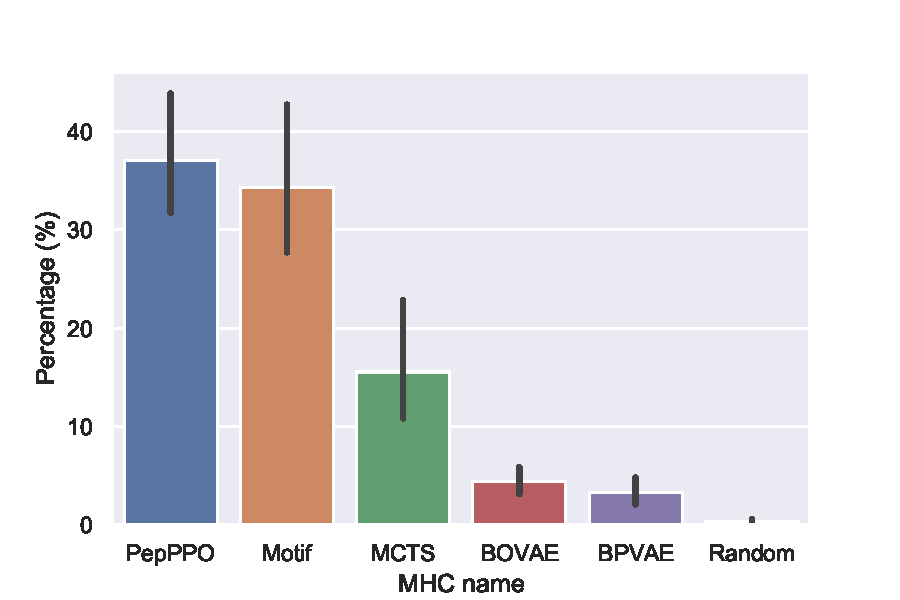
\includegraphics[width=\linewidth]{plots/mhc_avgresult_with_data.pdf}
		\caption{MHC Molecules with Data}
		\label{fig:avg_result_with_data}
	\end{subfigure}
	~~
	\begin{subfigure}[b]{.45\linewidth}
		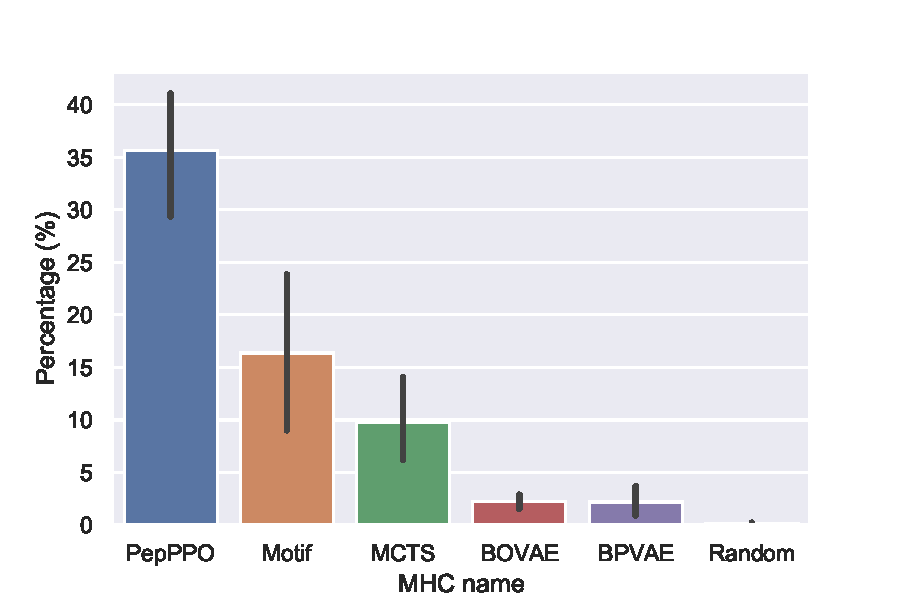
\includegraphics[width=\linewidth]{plots/mhc_avgresult_without_data.pdf}
		\caption{MHC Molecules without Data}
		\label{fig:avg_result_without_data}	
	\end{subfigure}
	\caption{Performance Comparison on Average Percentage of Qualified Peptides over 1K Peptides for MHC Molecules \
		with and without Data in the Dataset.}
\end{figure}

%%%%%%%%%%%%%%%%%%%%%%%%%%%%%%%%%%%%%%%%%%%%%%%%%%%%%%%%%%%%%%%%%%%%%%%%%%%%%%%%%%%%%%%%%%%%%%%%%%%%%%%%%%%%
\section{Experimental Results}
\label{sec:results}
%%%%%%%%%%%%%%%%%%%%%%%%%%%%%%%%%%%%%%%%%%%%%%%%%%%%%%%%%%%%%%%%%%%%%%%%%%%%%%%%%%%%%%%%%%%%%%%%%%%%%%%%%%%%

%===========================================================================================================
\subsection{Overall Comparison}
\label{sec:results:without}
%===========================================================================================================

We sampled a set of MHC Class I molecules with and without the data, and compared the performance of all the methods on generating
peptides bound to the MHC molecules.
%
Each method is used to generate 1K peptides for each MHC molecule.
%
Figure~\ref{fig:avg_result_with_data} and Figure~\ref{fig:avg_result_without_data} present the performance 
comparison on the generation of peptides bound to MHC molecules with and without data, respectively.
%
As shown in the figures, \pepppo achieves the highest percentages of qualified peptides (i.e., with presentation scores greater than 0.75)
among all the methods.
%
For the MHC molecule with the data, \pepppo outperforms the best baseline \pwm by about 3\%.
%
The good performance of \pwm on these MHC molecules could be due to that the frequency matrices derived from enough qualified peptides 
(i.e., 1.6K - 26K in the dataset) can accurately describe the distribution of qualified peptides of these MHC molecules.
%
The better performance of \pepppo over \pwm could demonstrate that \pepppo can learn the additional patterns of qualified 
peptides.
%
For MHC molecules without the data, \pepppo significantly outperforms the best baseline \pwm by about 20\%.
%
When the MHC molecules don't have enough qualified peptides in the dataset and are not similar with any other MHC molecules with the sufficient peptides, 
\pwm cannot find the position weight matrices from the dataset that could accurately describe the distribution of qualified peptides of these MHC molecules,
leading to the worse performance on generating qualified peptides.
%
Instead, \pepppo learns a common policy network to generate peptides bound to any random MHC molecules, and thus, achieves comparable performance 
on MHC molecules with the data (i.e., 36\%).
%
Generating qualified peptides for MHC molecules without the data is more important than that for MHC molecules with thousands of 
peptides known to be qualified.
%
Therefore, \pepppo could be used to generate quantified peptides of MHC molecules.

%===========================================================================================================
\subsection{Case Study}
\label{sec:results:case_study}
%===========================================================================================================

In Figure~\ref{fig:tsne}, we plotted four t-SNE plots of the generated qualified peptides in the above experiments for two MHC molecules HLA-A*02:01 and HLA-C*0602 with enough 
qualified peptides in the dataset and two MHC molecules HLA-A*11:04 and HLA-B*15:13 without.
%
From Figure~\ref{fig:case:hla-a0201} and Figure~\ref{fig:case:hla-c0602}, we observed that both \pwm and \pepppo can cover the space of qualified peptides populated by the existing 
qualified peptides (i.e., binding affinity $<$ 500) in the dataset.
%
This demonstrates that the generated qualified peptides of \pepppo have similar distributions with those in the dataset.

\begin{figure}[!t] 
	\centering
	\begin{subfigure}[b]{.48\linewidth}
	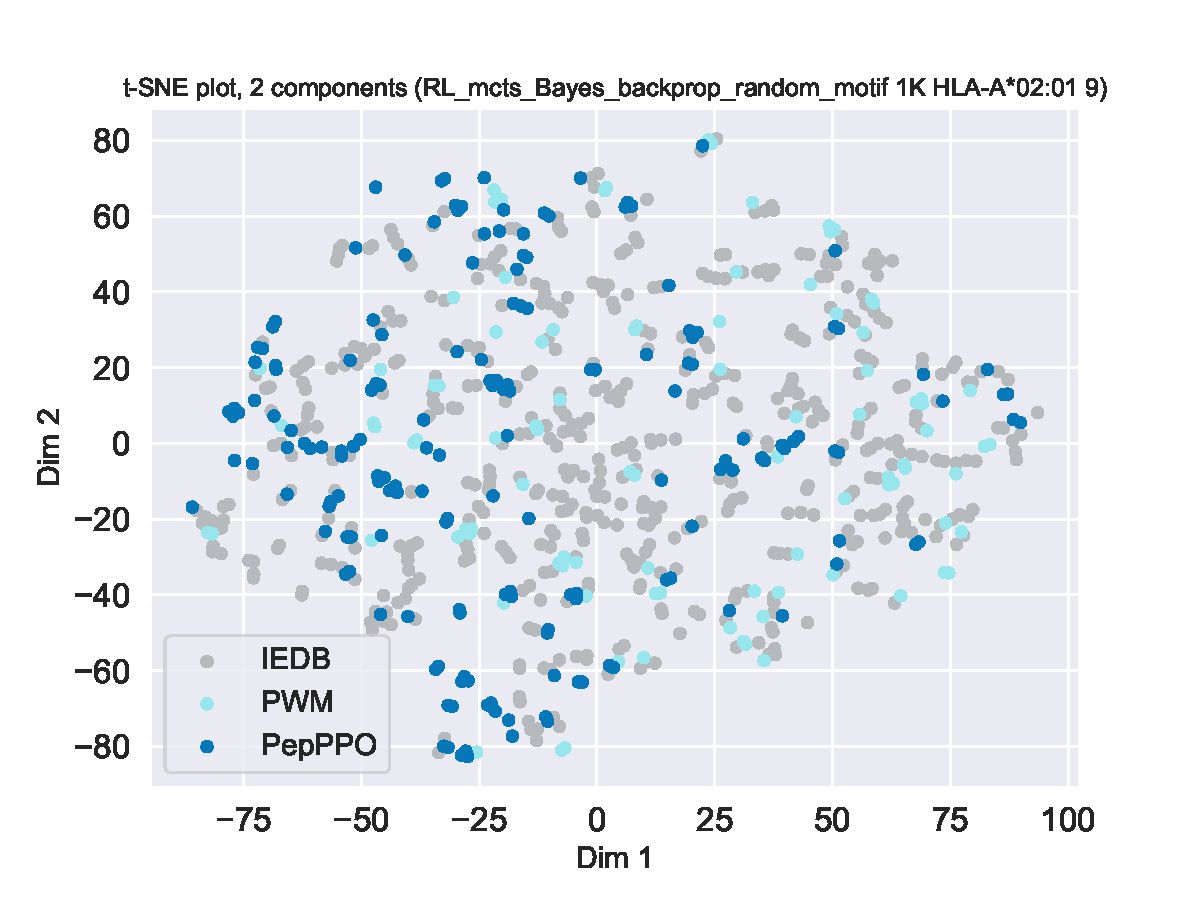
\includegraphics[width=\linewidth]{plots/HLA-A0201_RL_mcts_Bayes_backprop_random_motif_1K_9.pdf}
	\caption{HLA-A*02:01 with data}
	\label{fig:case:hla-a0201}
	\end{subfigure}
%	~~
%	\begin{subfigure}[b]{.48\linewidth}
%	\centering
%	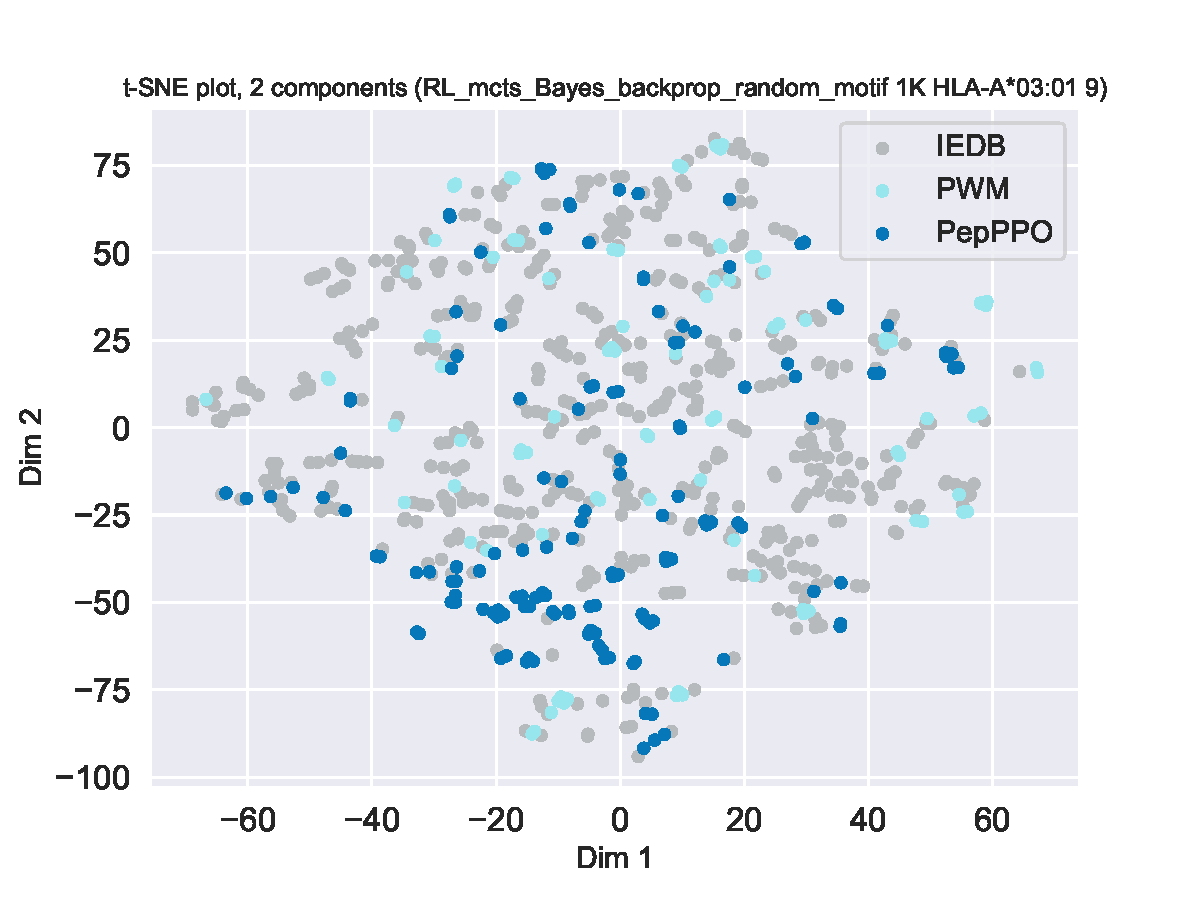
\includegraphics[width=\linewidth]{plots/HLA-A0301_RL_mcts_Bayes_backprop_random_motif_1K_9.pdf}
%	\caption{Average episode return, demonstrating }
%	\label{fig:avg_without}
%	\end{subfigure}
%    \\
%    \begin{subfigure}[b]{.48\linewidth}
%    	\centering
%    	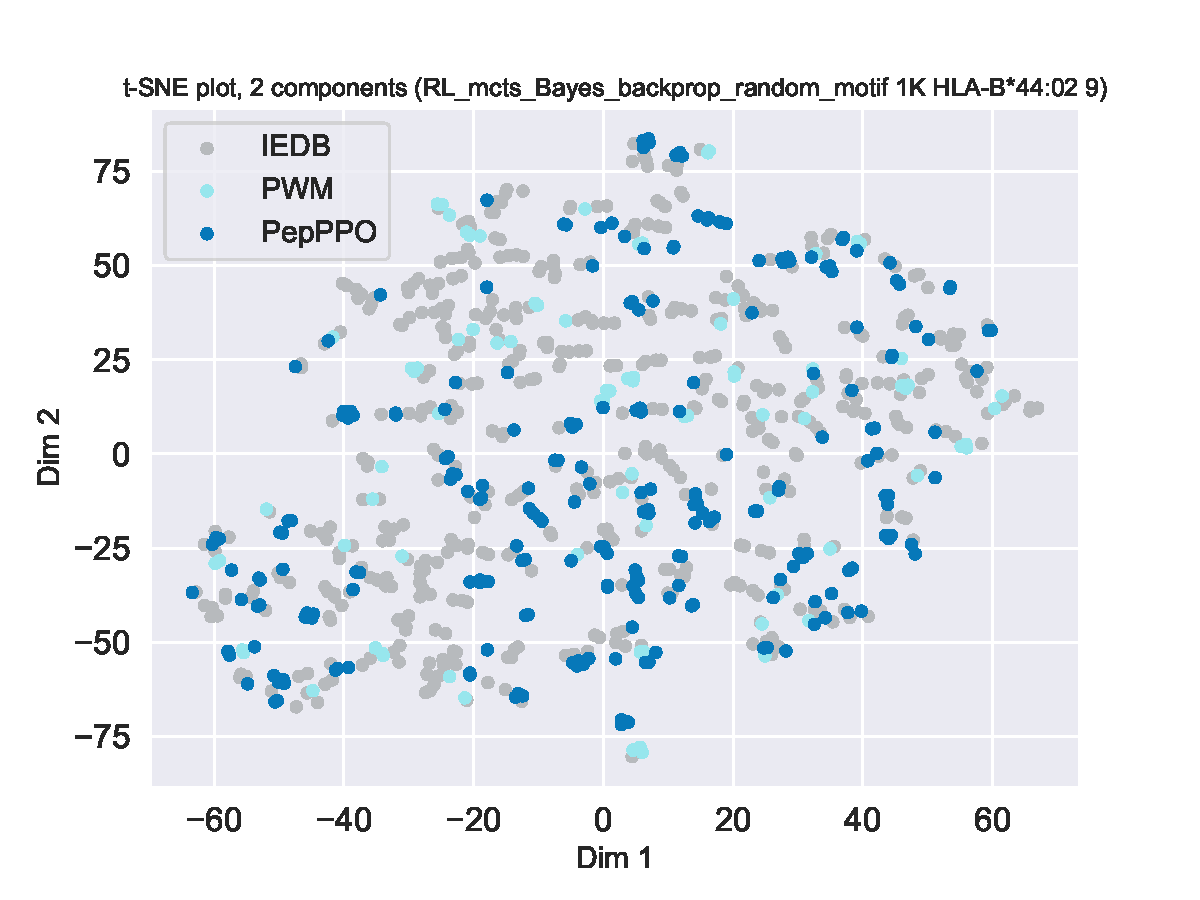
\includegraphics[width=\linewidth]{plots/HLA-B4402_RL_mcts_Bayes_backprop_random_motif_1K_9.pdf}
%    	\caption{Average episode return, demonstrating }
%    	\label{fig:avg_without}
%    \end{subfigure}
%    ~~
%    \begin{subfigure}[b]{.48\linewidth}
%    	\centering
%    	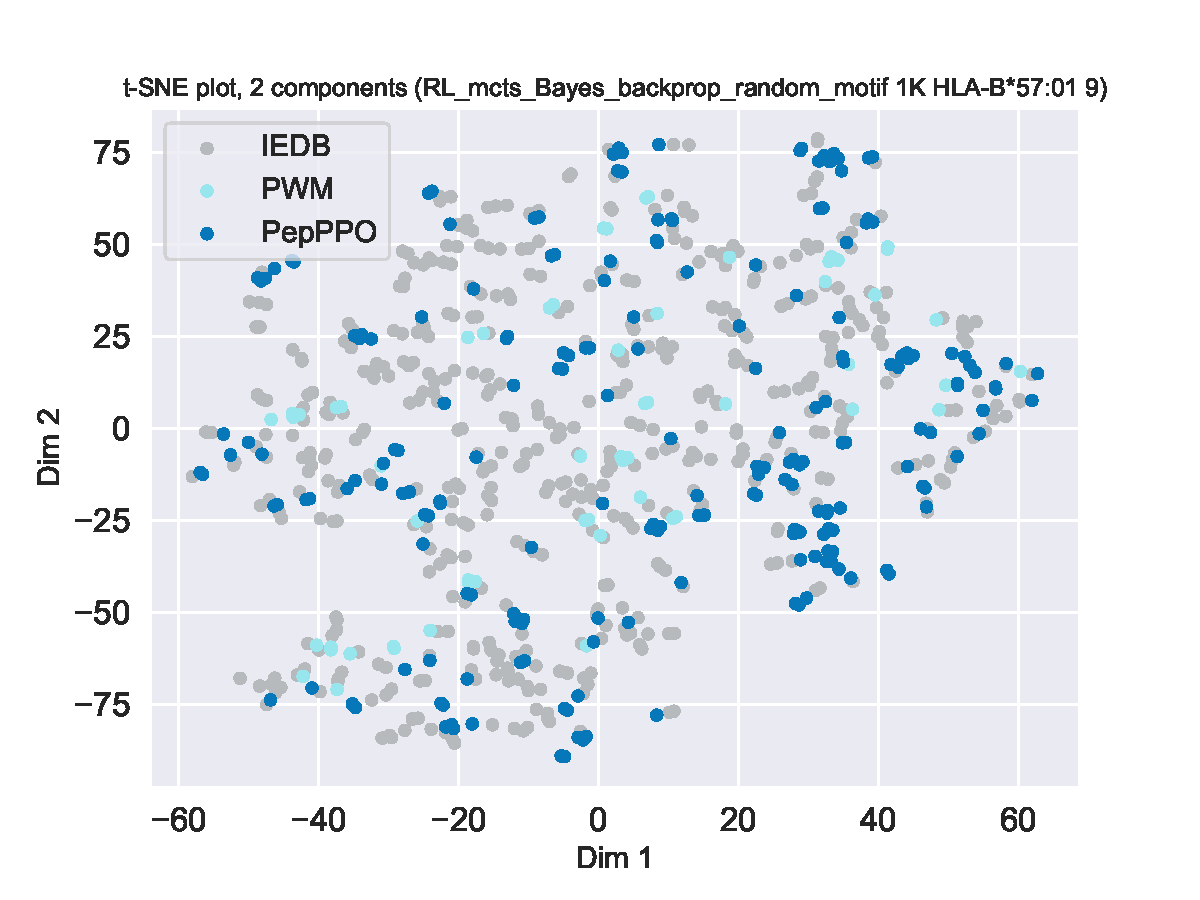
\includegraphics[width=\linewidth]{plots/HLA-B5701_RL_mcts_Bayes_backprop_random_motif_1K_9.pdf}
%    	\caption{Average episode return, demonstrating }
%    	\label{fig:avg_without}
%    \end{subfigure}
%    \\
%    \begin{subfigure}[b]{.48\linewidth}
%    	\centering
%    	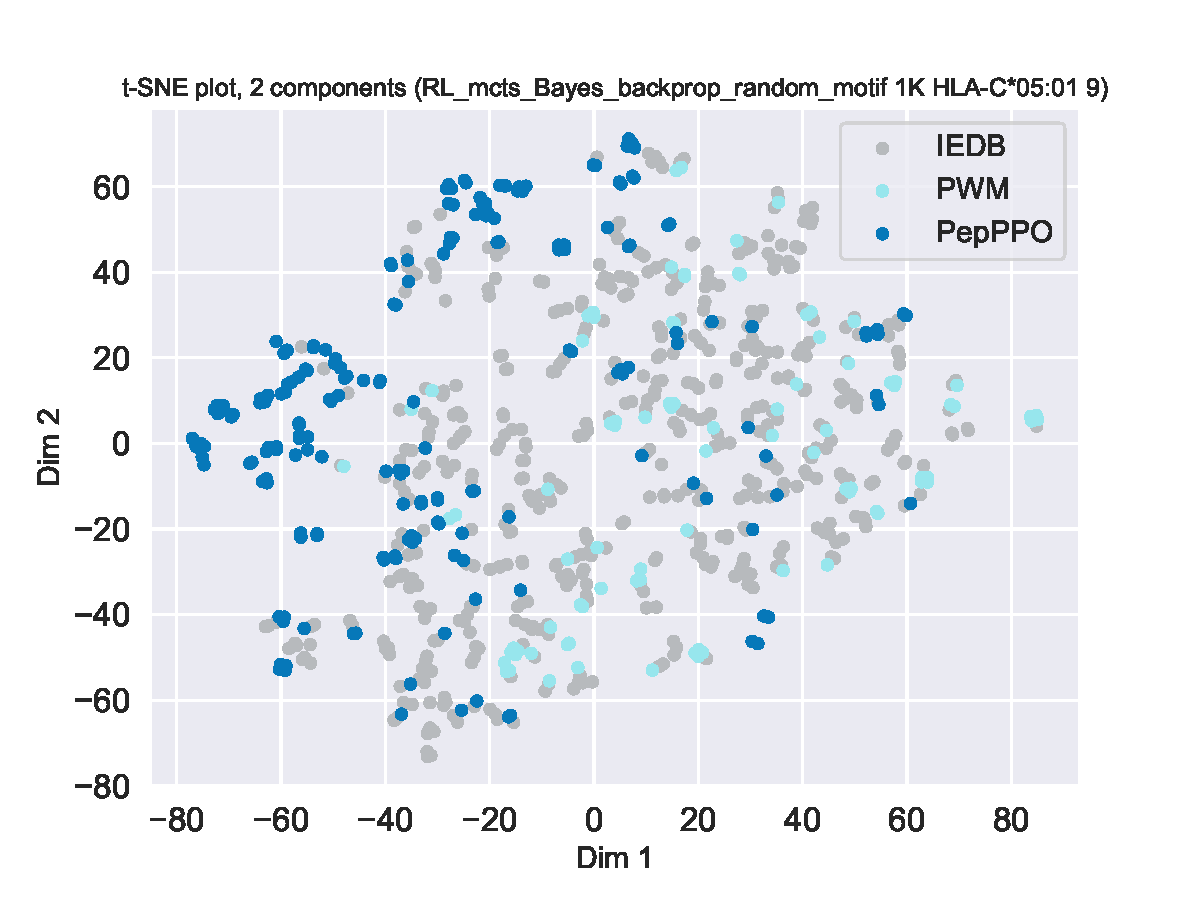
\includegraphics[width=\linewidth]{plots/HLA-C0501_RL_mcts_Bayes_backprop_random_motif_1K_9.pdf}
%    	\caption{Average episode return, demonstrating }
%    	\label{fig:avg_without}
%    \end{subfigure}
    ~~
    \begin{subfigure}[b]{.48\linewidth}
    	\centering
    	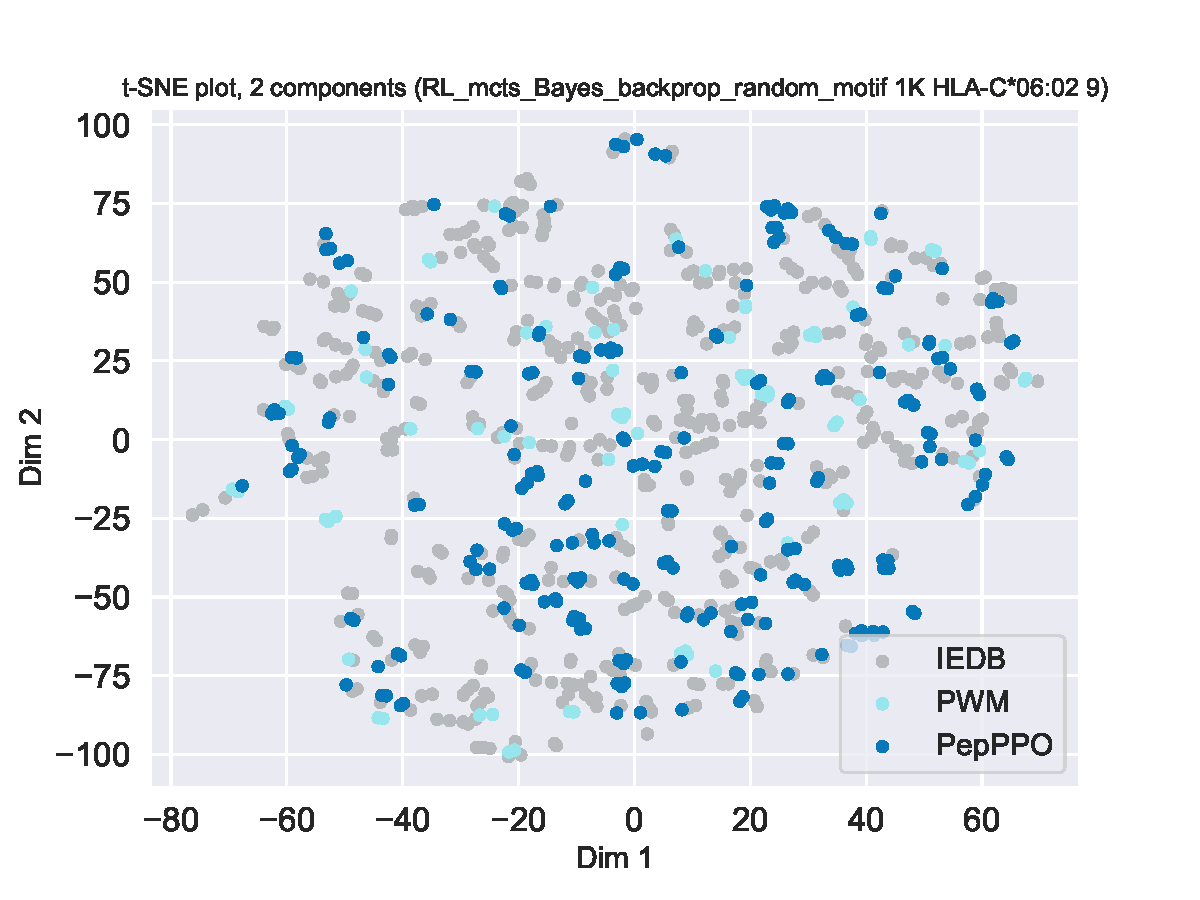
\includegraphics[width=\linewidth]{plots/HLA-C0602_RL_mcts_Bayes_backprop_random_motif_1K_9.pdf}
    	\caption{HLA-C*06:02 with data}
    	\label{fig:case:hla-c0602}
    \end{subfigure}
    \\
    \begin{subfigure}[b]{.48\linewidth}
    	\centering
    	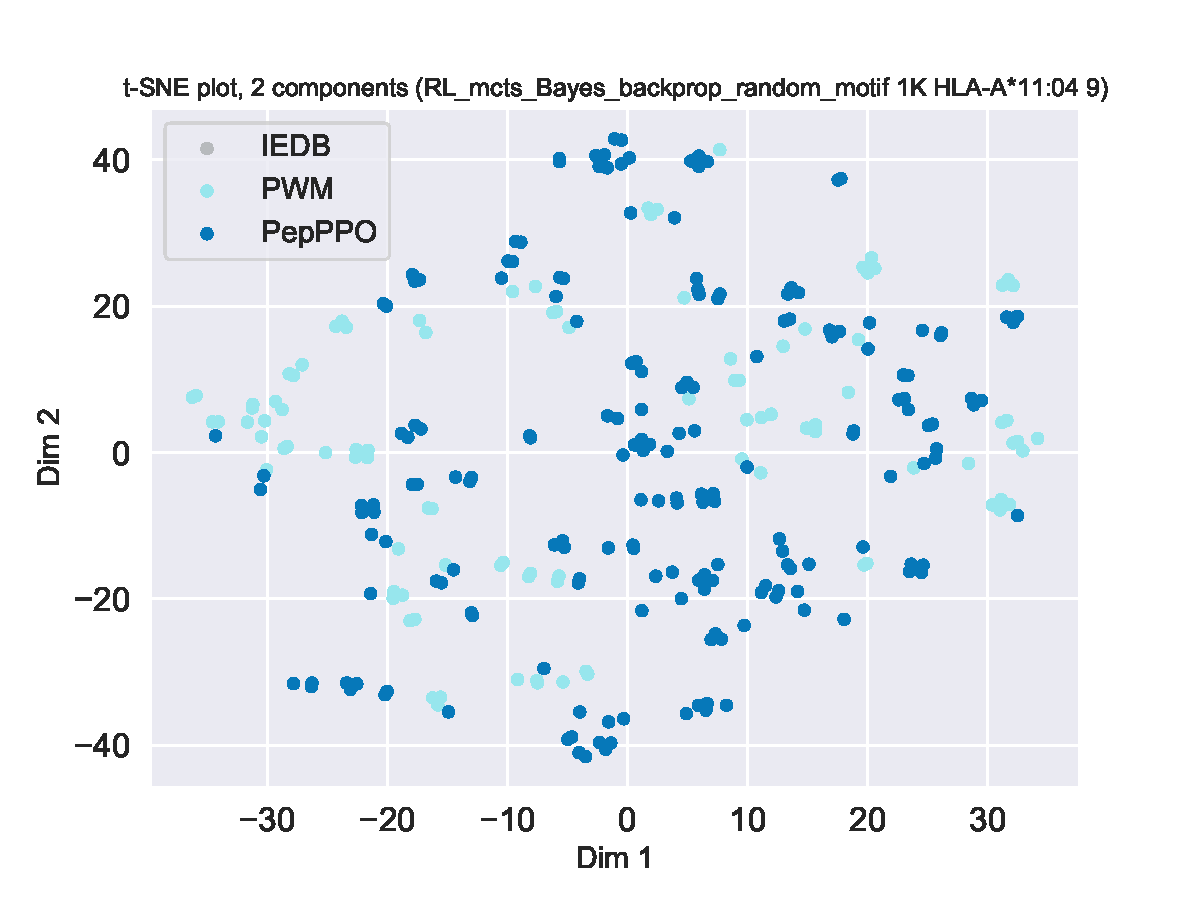
\includegraphics[width=\linewidth]{plots/HLA-A1104_RL_mcts_Bayes_backprop_random_motif_1K_9.pdf}
    	\caption{HLA-A*11:04 without data}
    	\label{fig:case:hla-a1104}
    \end{subfigure}
    ~~
    \begin{subfigure}[b]{.48\linewidth}
    	\centering
    	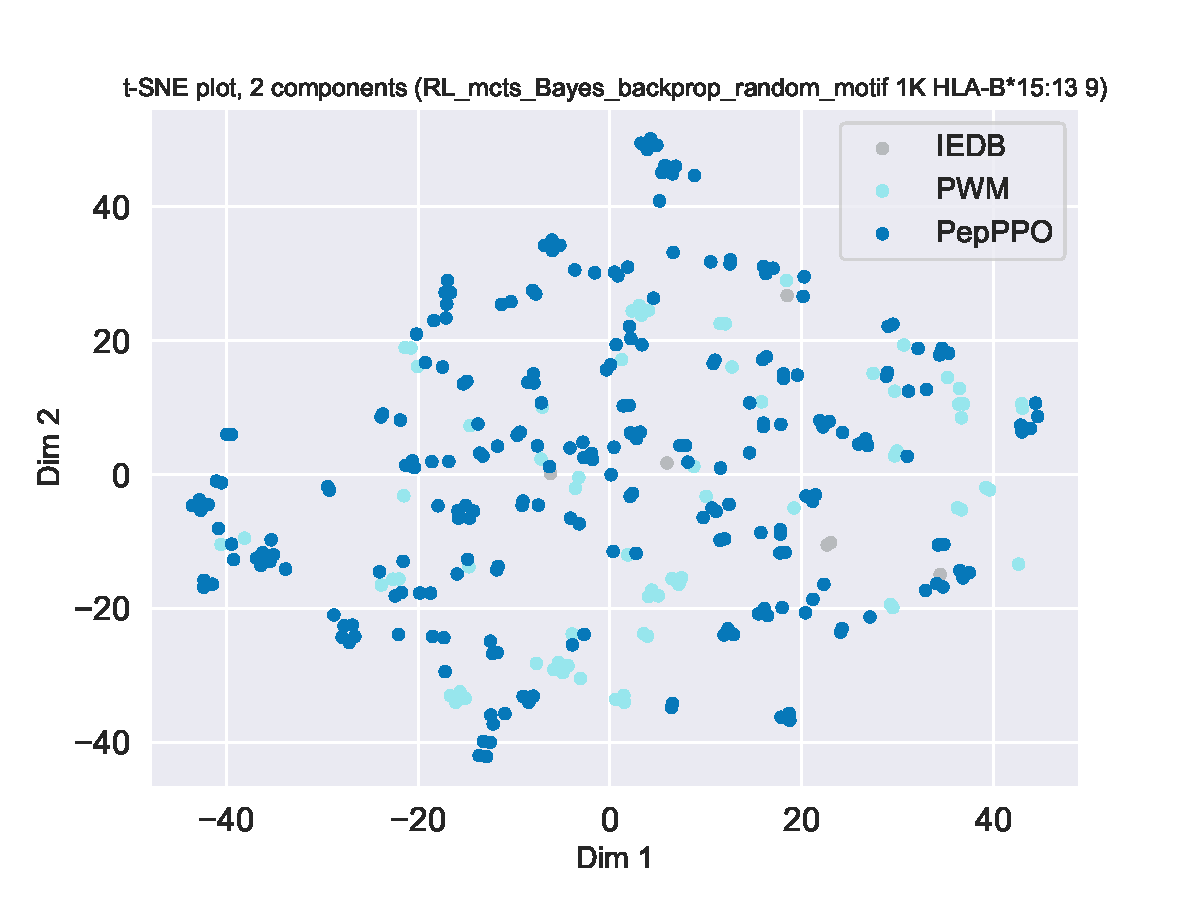
\includegraphics[width=\linewidth]{plots/HLA-B1513_RL_mcts_Bayes_backprop_random_motif_1K_9.pdf}
    	\caption{HLA-B*15:13 without data}
    	\label{fig:case:hla-b1513}
    \end{subfigure}
	\caption{t-SNE plot of the generated peptides for MHC molecule HLA-A0201 and HLA-C0602}
	\label{fig:tsne}
\end{figure}

%%%%%%%%%%%%%%%%%%%%%%%%%%%%%%%%%%%%%%%%%%%%%%%%%%%%%%%%%%%%%%%%%%%%%%%%%%%%%%%%%%%%%%%%%%%%%%%%%%%%%%%%%%%%
\section{Ablation Studies}
\label{sec:study}
%%%%%%%%%%%%%%%%%%%%%%%%%%%%%%%%%%%%%%%%%%%%%%%%%%%%%%%%%%%%%%%%%%%%%%%%%%%%%%%%%%%%%%%%%%%%%%%%%%%%%%%%%%%%

%===========================================================================================================
\subsection{Threshold}
\label{sec:dis:policy}
%===========================================================================================================




%===========================================================================================================
\subsection{Maximum Length of Steps}
\label{sec:dis:policy}
%===========================================================================================================

\begin{figure}
	\begin{subfigure}[b]{.48\linewidth}
		\centering
		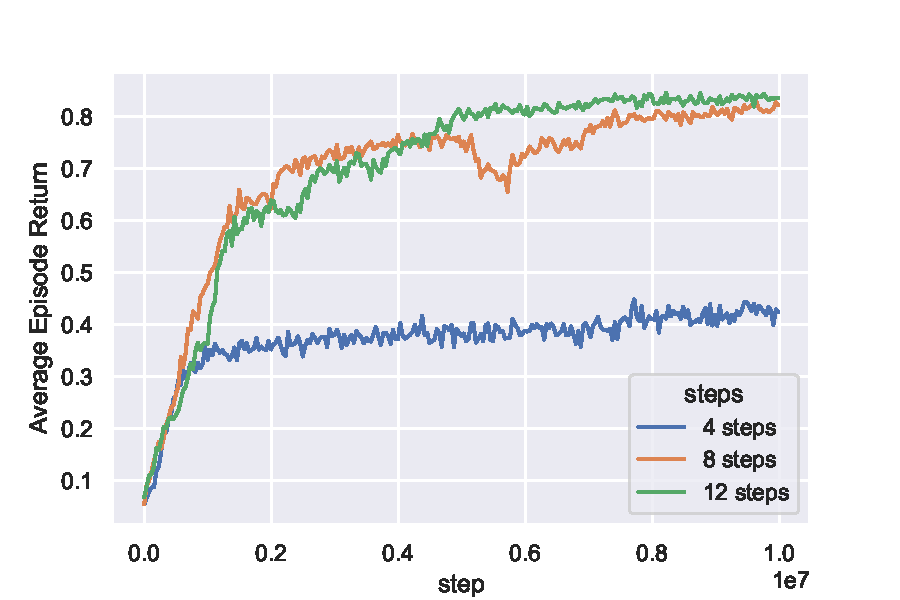
\includegraphics[width=\linewidth]{plots/step_reward.pdf}
		\caption{Average Final Presentation Scores of RL agents}
		\label{fig:step:reward}
	\end{subfigure}
	~~
	\begin{subfigure}[b]{.48\linewidth}
		\centering
		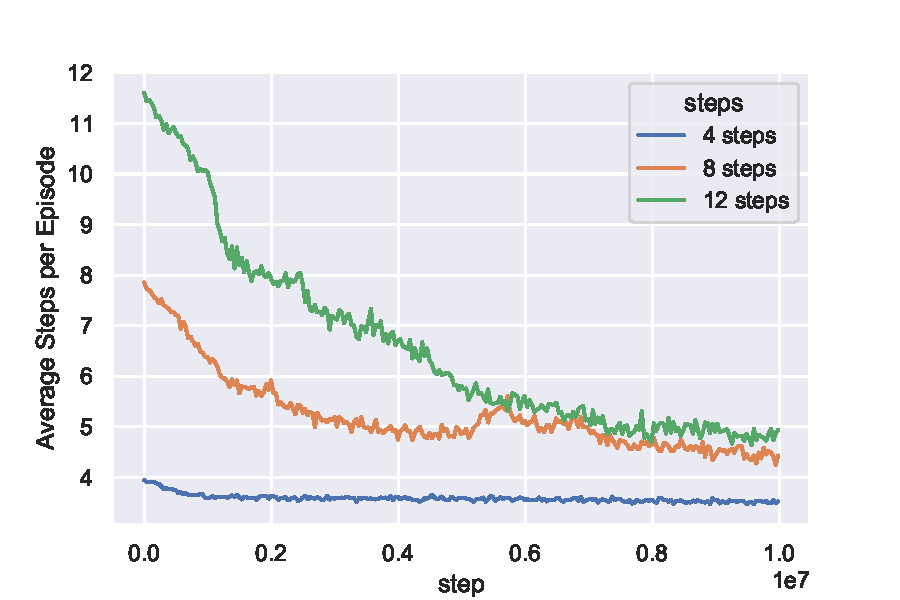
\includegraphics[width=\linewidth]{plots/step_length.pdf}
		\caption{Average Episode Length of RL agents}
		\label{fig:step:length}
	\end{subfigure}
	\caption{Comparison of RL Agents with Different Maximum Steps}
	\label{fig:step}
\end{figure}

Figure~\ref{fig:step} presents the performance comparison of RL agents with the maximum 4 steps, 8 steps and 12 steps
on the average presentation scores (Figure~\ref{fig:step:reward}) and the average length for each episode (Figure~\ref{fig:step:length}).
%
Figure~\ref{fig:step:reward} shows that 


%%%%%%%%%%%%%%%%%%%%%%%%%%%%%%%%%%%%%%%%%%%%%%%%%%%%%%%%%%%%%%%%%%%%%%%%%%%%%%%%%%%%%%%%%%%%%%%%%%%%%%%%%%%%
\section{Discussion}
\label{sec:dis}
%%%%%%%%%%%%%%%%%%%%%%%%%%%%%%%%%%%%%%%%%%%%%%%%%%%%%%%%%%%%%%%%%%%%%%%%%%%%%%%%%%%%%%%%%%%%%%%%%%%%%%%%%%%%

%===========================================================================================================
\subsection{Peptide Mutation Policy}
\label{sec:dis:policy}
%===========================================================================================================

Two examples, one with data and another without data. Plot the distributions of the predicted actions.

%%%%%%%%%%%%%%%%%%%%%%%%%%%%%%%%%%%%%%%%%%%%%%%%%%%%%%%%%%%%%%%%%%%%%%%%%%%%%%%%%%%%%%%%%%%%%%%%%%%%%%%%%%%%
\section{Conclusion}
\label{sec:conclusion}
%%%%%%%%%%%%%%%%%%%%%%%%%%%%%%%%%%%%%%%%%%%%%%%%%%%%%%%%%%%%%%%%%%%%%%%%%%%%%%%%%%%%%%%%%%%%%%%%%%%%%%%%%%%%

\bibliography{bib}
\bibliographystyle{abbrv}

\end{document}